\documentclass[11pt,a4paper]{article}
\usepackage[margin=1.0in]{geometry}
\usepackage{url}
\usepackage{graphicx}
\graphicspath{ {./image/} }

%opening
\title{\vspace{5em}{\Huge Chord and DHT}}
\date{\vspace{-8em}{\Large 15 pages}} %Make edit here

\author{\vspace{5em}\\\textbf{\Large Liu Linlin}\\A0078051J \and \vspace{5em}\\\textbf{\Large Vipul Sharma}\\A0178385M \and \vspace{5em}\\\textbf{\Large Anshul Aggarwal}\\A0191501R}



\begin{document}
    
    \maketitle
    \newpage
    
    \begin{abstract}
        We discuss the development of distributed storage systems, primarily focusing on Distributed Hash Tables (DHTs), which are used for lookup in such systems. Designing such a large scale system can be quite hard, and we describe some design techniques and goals, their pros and cons, and the optimal scenarios for these design choices. We also look at the evolution of such systems over the past couple of decades, their advantages and limitations, and some promising future directions for the field as a whole.
    \end{abstract}
    
    \section{Introduction}
    
    Over the last two decades, the need for storing and sharing large amounts of data for quick and easy availability to a large number of users over networks has gone up substantially, both in business and consumer space. Such environments require scalable key-value storage systems. Services such as Apache Cassandra \cite{Cassandra} and Amazon's DynamoDB\cite{DynamoDB} provide scalable, reliable key-value storage systems for organizations, while BitTorrent based Distributed Hash Tables (DHTs) store metadata and enable file sharing among hundreds of millions of users through peer-to-peer protocols.
    
    All of the above systems are \textit{distributed} in nature. Such de-centralized or distributed storage systems allows a number of advantages over traditional centralized systems, such as support for scalability, more robust automatic load balancing, and improved data availability and reliability through the use of efficient replication techniques. Such systems may have some other features, including but not limited to permanence, anonymity, selection of closest servers, and distributed searching. They are also easier to design, implement and debug over a large scale. This is precisely the reason such storage systems now find use in a large number of applications.
    
    One important limitation to consider while using such de-centralized systems for applications is that such systems can be somewhat difficult to customize for the particular application's needs, even if the changes required are conceptually simple. For example, the authors of Vanish \cite{geambasu2009vanish} --- a security oriented distributed application, state that making small, application-specific policy and parameter changes in a popular DHT system is a time and resource intensive process.
    
    In this paper, we discuss several designs of DHT systems and protocols, and some potential future research directions based on the current state-of-the-art.
    
    \subsection{Distributed Hash Tables (DHTs)}
    
    These are a type of highly-distributed storage systems, allowing key-based object lookup in a dynamic, scalable network environment. The objects mapped by keys can be anything --- documents, addresses or even arbitrary data.\cite{ChordStoica} The object data corresponding to the access \textit{key}, called \textit{value}, is kept at storage nodes whose identification information is generally hashed to form the key. For better reliability and availability of data, many DHTs replicate node data, or values to the node's neighbours.\cite{PastryRowstron}.
    
    \section{DHT Design}\label{DHTDesign}
    
    \subsection{Interface}
    
    For designing any DHT system, certain capabilities or design parameters must be chosen. Three broad categories of interfaces have been developed over time, and they provide three distinct capabilities for a given input key, as described below. It is of note that they however work in conflicting ways, with generalized designs being complex,  sacrificing simplicity and ease-of-use. \cite{dabekp2p}
    
    \subsubsection{Routing} This interface provides access to the DHT node corresponding to the input key, as well as to all the nodes in the routing path, in order of access to reach the target node. 
    
    This is the most generalized interface. Clients can invoke arbitrary code at all nodes --- be it the target node or the nodes in the routing path. This interface has been used in implementing multicast \cite{SplitStreamCastro} and anycast \cite{TapestryZhao} based on DHT.
    
    \subsubsection{Lookup} This interface only gives access to the DHT node corresponding to the input key.
    
    As compared to the routing, the lookup interface model is less flexible and generalized, as it only allows clients to invoke code only at the target nodes. Derivations of this model have been used in packet forwarding \cite{IIIStoica}, file systems \cite{IvyMuthitacharoen,CFSDabek} and query processing. \cite{PierHuebsch}
    
    Both lookup and routing allow application-specific code to execute on DHT nodes.
    
    \subsubsection{Storage} This interface directly allows \textit{get} operation on keys, as well as \textit{put} operation on key-value pairs by routing to the DHT node corresponding to the input key. This does not expose any other interface in the process.
    
    This model is the least versatile, as it does not allow any application specific code to execute on any node, instead only allows \textit{get}/\textit{put} operations to be called. However, this model is very easy to implement and support, as the DHT infrastructure does not have to bother about supporting unknown application-specific procedures.
    
    \subsection{Properties and Goals}
    
    Any DHT system is designed keeping some design properties and goals in mind. These goals can affect the structure of the DHT system, and may include choosing the right interface model as described above. This may lead to various limitations, or hold several advantages based on the type of applications the DHT system is targeting. A few design goals that may be considered for some applications are described below. \cite{DHTWehrle}
    
    \subsubsection{Consistency}\label{consistency}
    
    The system should be able to handle variable-latency and lossy network connections, communication failures, and uncontrolled system membership changes, where clients may join or leave the system without any previous indication. Despite all of the above inconsistencies, the system should be able to keep the data available and uncorrupted.
    
    \subsubsection{Scalability}
    
    The system should be able to dynamically scale to large number of nodes, with differing computational capabilities, network bandwidth and churn rates, without significant or any changes in the architecture.
    
    \subsubsection{De-centralization}
    
    The nodes are not centrally coordinated and collectively form the DHT system, handling all operations in a de-centralized way.
    
    \subsubsection{Adaptability}
    
    The system should be ``self-optimizing'' to changing operational conditions. For example, it should be able to maintain a balance of availability and performance even as it scales. Or, it should be able to adapt to network architecture changes, maintaining the required performance levels at all time.
    
    \section{Foundations of Distributed Storage}
    \subsection{Pastry} \label{pastry}
    Pastry \cite{PastryRowstron} is an object location and routing protocol for peer-to-peer Internet applications. Pastry is decentralized, which means all the nodes in the network are equal so that no centralized sever is required to facilitate this. All the nodes in Pastry coordinate with each other to handle many other functions apart from object location and routing, including adding or removing a new node, node failures and so on.
    
    Pastry has good network locality property and tries to minimize message routing distance, which makes it scalable and efficient for very large networks. Many applications have already been developed using these capabilities of Pastry in different ways. One example is PAST, which use Pastry for file storage and replication. SCRIBE is another example, which use Pastry for message publish/subscribe.
    
    \subsubsection{Pastry Design and Parameters}
    
    The design of Pastry is based on a decentralized network of nodes. Each node in the peer-to-peer network is randomly assigned a 128-bit node identifier when it joins the network, which denoted by nodeId. We try to make sure all the assigned nodeId are uniformly distributed in the 128-bit nodeId space, one way to do this is to use a cryptographic hash function. We notice that the nodeId space here is circular, which is very similar to Chord, another design of distributed hash table that will be discussed later in this paper.
    
    There are two configurable parameters in Pastry. b is the length of bits used to represent each digit of nodeId or key, a typical value is 4. So nodeIds and keys can be thought of as a sequence of digits of base \(2^{b}\).Assume there are N nodes in the network, the upper bound of the number of steps to route any message will be \(\log_{2^b} N \). The other configurable parameter is L, which is used to determine the size of adjacent nodeIds (L/2) to check when routing messages.
    
    Each node in Pastry maintains its node state, including a routing table, a neighbourhood set and a leaf set. Only leaf set and routing table are used for message routing. The neighbourhood set is used for exchanging information about nearby nodes. For example, a node attempts to contact each member of the neighbourhood set periodically to detect node failures. 
    
    \begin{figure}[h]
        \centering
        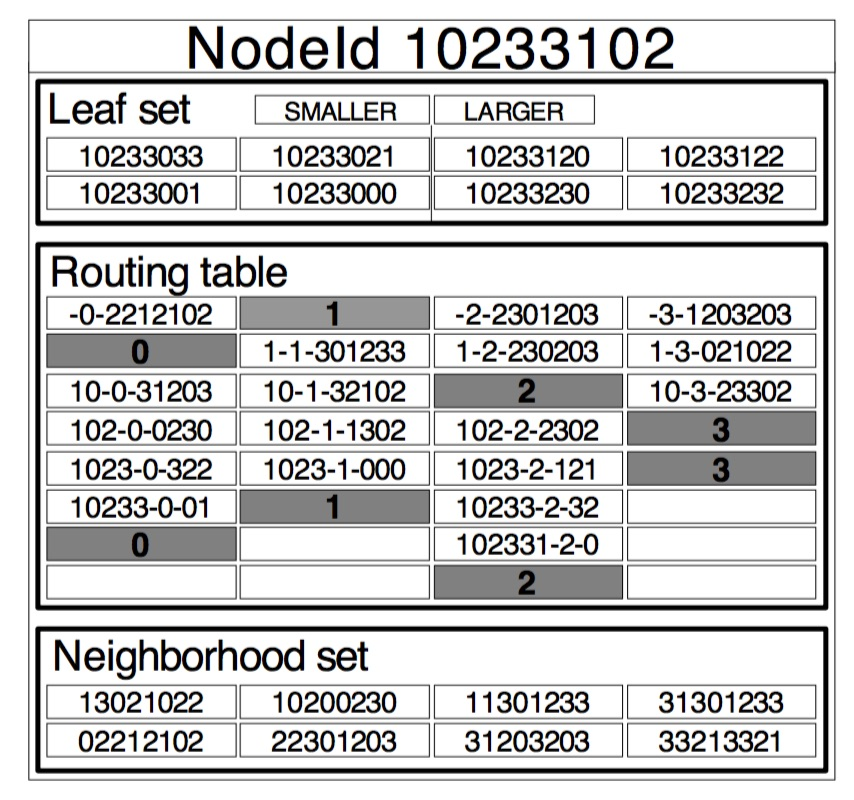
\includegraphics[scale=0.3]{image/pastry_node_state.jpg}
        \caption{Pastry Node State Table}
        \label{pastrynst}
    \end{figure}
    
    Figure \ref{pastrynst} is an example that shows the state of a node with nodeId 10233102. The leaf set contains the nodeIds that are closest to the current one. Routing table contains \(\log_{2^b} N \) rows and \(2^{b}\) columns. Each entry contains information of a node that is potentially close to the current one. We only show each entry’s nodeId in the table above. Their nodeId is divided into three parts: common prefix with the present nodeId, next digit, the rest part of the nodeId. Length of common prefix on each row is the same as the entry’s row index, starting from 0. Next digit on each row is from 0 to \(2^{b}-1\), which ensures that the nodeIds on each row is uniformly distributed.
    
    \subsubsection{Pastry Routing}
    When a new key D arrives at node A, we check whether D equals to A first. If D does not equal to A, we can follow the below steps to route message. In each step, Pastry tries to route the message to a node that is closer to D.
    
    Step 1: Check whether D is within the range of A’s leaf set. If so, route D to the node with minimal distance from this leaf set. Otherwise go to Step 2.
    
    Step 2: Check the length of the share prefix of A and D, denoted by \(l\). Check the \(l\)th digit of D, denoted by \(D_l\). Then go to row l of the routing table, check whether the entry in column \(D_l\) exits or not. If it exits, then rout to that entry. Otherwise go to Step 3, which is relatively rare.
    
    Step 3: Go though the nodes in leaf set, routing table and neighborhood set, and route the message to any node that is closer to D.
    
    \subsubsection{Pastry Node Arrival and Departure}
    When handling node arrival, Pastry can also use the above procedure to find an existing node that is closest to the new one, and then copy its node state and make minimal updates. After initialize its node state, the new node send information to each node in its neighborhood set, leaf set, routing table for them to update their node state accordingly. When handling node departure, the neighborhood nodes can detect failure and update their node state.
    
    \subsection{Chord} \label{chord}
    Chord \cite{ChordStoica} is another object location and routing protocol for peer-to-peer Internet applications. It also uses a circular node identifier space, which is similar to Pastry. However, their routing procedure are very different. Pastry uses the closest nodes to store data, while Chord uses the closest successor instead. Each node of Chord maintains information only about \( O(log N) \) other nodes. All lookups can also be resolved by \( O(log N) \) routing messages.
    
    \subsubsection{Chord Design}
    
    \begin{figure}[!htbp]
        \centering
        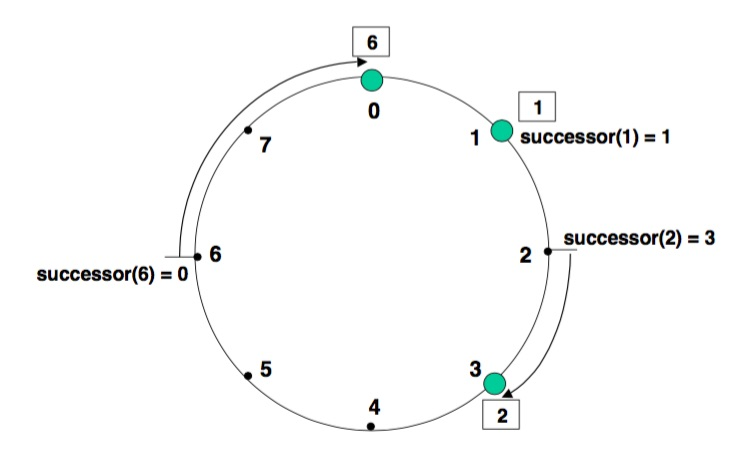
\includegraphics[scale=0.4]{image/chord.jpg}
        \caption{Chord}
        \label{fig:chord}
    \end{figure}
    
    Figure \ref{fig:chord} shows how successor of Chord works. Each node in Chord is assigned with an identifier using a hash function, they are ordered in a circular network by the value of identifier modulo \( 2^m \). m here is a parameter which determines the size of the circular network, which is \( 2^m \). For any key k in the identifier space, successor(k) is the first node available in the circular network clockwise from k.
    
    In this example, there are three nodes at 0, 1, 3 respectively. When we locate the successor of 6, we check whether there is any node at position 6 first. Since there is no node available at position 6, we move clockwise until we find the first node. Therefore, the successor of node 6 is located at position 0.
    
    \subsubsection{Chord Routing}
    
    Compared with Pastry, the routing procedure of Chord is more straightforward. Chord uses finger table to assist node location and message routing. Node X’s finger table maintains information about the successor nodes of identifier \( (X + 2^i )\ mod \ 2^m \), where \( i = 0, 1, ... , m-1 \). We can see that each node of Chord maintains information only about \( O(log N) \) other nodes. When a new key A arrives at node D, we will follow the below steps to route this message.
    
    Step 1: Check whether A falls between any node identifier and its successor in D’s finger table. If so, the successor is the node we are looking for. Otherwise got to Step 2.
    
    Step 2: Check the node that most closely precedes A in D’s finger table. Route A to that node.
    
    As we can see, every step in the routing procedure moves the key closer to node we are looking for in clockwise direction. 
    
    \subsubsection{Node Arrival and Departure}
    
    Chord also handles node arrival and departure in a very elegant way, since we only need to point to its successor for message routing. The whole network will only need \( O((log N)^2) \) messages to update other nodes’ finger tables.
    
    \section{Advances in Distributed Hash Tables}
    
    \subsection{OpenDHT} \label{opendht}
    
    One of the most significant advancements in the Distributed Hash Table space came with the introduction of OpenDHT \cite{OpenDHTRhea}. This was one of the first free, public DHT service. In short, the system consists of infrastructure nodes, and the client nodes exist outside the system. Client nodes are able to run applications that invoke the OpenDHT service using Remote Procedure Calls (RPCs). An infrastructure node participates in routing and storage, along with acting as a gateway for Client RPCs.
    
    OpenDHT has a significant advantage in that applications do not have to bother about the DHT deployment. This allows the architecture and operation of OpenDHT to be simple and the system easy to use, as no application specific code is part of the DHT system. Thus the \textit{storage interface model} was chosen for the design of this system, as discussed above in section \ref{DHTDesign}.
    
    \subsubsection{Design properties}
    
    OpenDHT has been designed to make applications using it easy to write. It provides a \textit{get}/\textit{put} interface for the same, as required by a storage interface model. 
    
    Secondly, OpenDHT does not restrict key choices, as it does not require any particular relationship between the keys and corresponding values. This is because some applications like a prefix-hash tree \cite{PHTRamabhadran} cannot function with such a restriction.
    
    On the consistency front, OpenDHT only achieves eventual consistency. It is possible that due to some network or processing capability limitation on the node end, inconsistencies as discussed above in section \ref{consistency} can occasionally occur.
    
    \subsubsection{Storage policy}
    
    As observed in \cite{PalimpsestRoscoe}, any such system allowing persistent storage, as found in traditional file systems, the system eventually is accumulated with \textit{orphaned data}. So, a technique where new data pushes out the old data as the disk gets full, a la a revolving door, was proposed. \cite{PalimpsestRoscoe} Taking inspiration from this, in OpenDHT, for any client to maintain its data, it must re-put data on the DHT periodically so that it is never flushed. In contrast to \cite{PalimpsestRoscoe}, where clients need to monitor load to know when to re-put data, OpenDHT uses a time-to-live (TTL) mechanism, where there is a set time after which the client must re-put data.
    
    %The following paragraph is a new addition, dated 6 Nov.
    
    \paragraph{Storage allocation} OpenDHT implements a per-disk storage allocation model of fairness, where each client gets a fair allocation of every disk in the system. To decide allocation among competing clients, and also prevent per-client starvation, OpenDHT tries to equalize the rate of commitments (each commitment is equivalent to the product of \textit{put} size and its TTL) across clients, instead of allocation based on the total commitments made by a client. The authors implement a Fair Space-Time (FST) algorithm for this purpose.
    
    
    \subsubsection{Interface}
    
    A \textit{put} in OpenDHT has a unique identification based on a triple, which has a key, a value and the SHA-1 hash of a random secret chosen by the client. Multiple \textit{puts} with same key and value are stored. If even the secret hash is same, then the TTL refreshes for the existing \textit{put}.
    
    A \textit{get} takes a key and returns corresponding values, secret hashes and TTLs. Removing a value requires the client to reveal the secret along with the key for which the \textit{put} holds the hash. Change in value is just a combination of removing a value and a fresh \textit{put}.
    
    %The following subsection is a new addition, dated 6 Nov.
    
    \subsubsection{Making OpenDHT more flexible}
    
    Since OepnDHT is based on the storage interface model, it can be quite inflexible to preserve simplicity, as discussed in section \ref{DHTDesign}. However, this means that there are still quite a few application scenarios which are not supported, as they explicitly require somewhat more sophisticated designs offered by interfaces like \textit{lookup}. To circumvent this limitation, OpenDHT implements a client side library called ReDiR, that provides functionality similar to the \textit{lookup} interface.
    
    The lookup interface allows nodes to have application specific functionality, which is returned by the lookup function. OpenDHT does not allow nodes inside the DHT to have this, but via ReDiR, allows secondary, application-specific nodes outside the DHT to host application specific code. Clients can then use OpenDHT using ReDiR to route by key among these nodes. ReDiR, however, interacts with OpenDHT using the standard \textit{get}/\textit{put} API, thereby leaving the DHT system unaffected.
    
    \subsection{Comet} \label{comet}
    
    Comet \cite{CometGeambasu} is an advanced distributed key-value storage system which comes with several advantages (and a few disadvantages) over other distributed storage systems like Amazon S3, DynamoDB, Apache Cassandra. In Comet, these key-value pairs are stored with some additional code and are collectively called as Active Storage Objects (ASOs). This additional code is nothing but a set of handlers which are invoked at the time of common storage events like GET, PUT, DELETE and Timer events. The value, along with the data produced by the handlers, is also known as the state of the ASO. For example, whenever a client performs a GET operation to fetch some value, the ‘onGet’ handler is called. This handler can then perform various operations and store the resulting data in its state. The application specifies the initial state and handlers for an ASO and stores it via PUT operation.
    
    The goal for an ASO is to perform following tasks
    
    \begin{itemize}
        \item Gather statistical data like number of GET and PUT operations.
        \item Logging the IP addresses of the client nodes which accessed the value.
        \item Perform Time based operations, like deleting itself or synchronizing with other ASOs with similar key.
        \item Choose the location to store based on node’s location in the network.
        \item Control data replication.
        \item Provide behavioral information about the system.
        \item Implement access control policies.
    \end{itemize}
    
    \subsubsection{Relevance and Aim}
    
    The main aim of Comet is to be flexible and cater the varying requirements of applications for their data storage. Multiple applications can share a single Comet instance and configure its own storage elements to suit the requirements, unlike the scenario where they must run separate instances. The configuration can include different access methods, access control protocols, replication factor, security policies and lifetimes of their storage objects.
    
    Other primary goals include isolation and safety of the client nodes and performance of the system.
    
    \subsubsection{Trusted environment}
    
    To provide an isolated and secure environment, Comet enforces certain restrictions. They are described as follows.
    
    \begin{itemize}
        \item	An ASO should not be aware of other ASOs present on the same node. The APIs are designed in such a way to only allow communication between ASOs with the same key.
        \item	The ASO handlers should be able to modify only its own value. To ensure this, the ASO APIs are made restrictive to not allow access to any sensitive data which can result in an attack.
        \item	An ASO cannot send arbitrary messages to other ASOs over the network.
        \item	An ASO can consume only limited memory and CPU resources. This is taken care by the runtime system which impose these restrictions through sandboxing.
        
    \end{itemize}
    
    There is no notion of trust between the operating nodes which form a distributed storage system. To ensure safety, the Comet prototype is sandboxed based on a language called Lua \cite{LuaIerusalimschy}. This light-weight language has a small number of data types and programming constructs, and the bytecode it produces is relatively smaller in size and can be easily sandboxed. The Runtime, which implements the security policies and handle ASO invocations, exposes a set of APIs for the ASOs to interact with the environment outside its sandbox. These APIs include fetching the system time (helpful for timer events), getting node’s external IP address (to log it in the history), deleting itself (requirement for secure applications like Vanish \cite{geambasu2009vanish}) and a few others.
    
    \subsubsection{Storage in Comet}
    
    There are a range of storage behaviors which are supported by Comet for various application needs. They are listed as under.
    \begin{itemize}
        
        \item	The replication factor for ASOs can be configured based on the application’s requirements. To implement this, the ‘onTimer’ handler can be invoked periodically to determine a list of good nodes based on the ASO’s key and store its replica on them. Another useful strategy could be to replicate only when the number of replicas fall down below a certain number.
        \item	Various strategies can be implemented to access the stored data. ASOs can be configured to self-destruct after a specified period of time or they can be read only for a limited duration, which is a common practice for security-centric applications. This can be implemented by recording the system time on creation and then setting a timer. 
        \item	ASOs can also limit the number of GET and PUT operations which can be used as synchronization objects between producers and consumers.
        \item	ASOs can implement a publish-subscribe model in which clients can subscribe to an ASO and they will receive a notification when its value changes.
        \item	ASOs can restrict the access to its value using a password protection. Clients will have to pass the encrypted password as an argument to retrieve the value.
        \item	ASOs can provide instrumentation data and measurements about the DHT. This can be done by nodes inside (with more accuracy) and outside the system. This data can be used for debugging purposes after consolidating the access list from all the replicas.
        \item	Comet can be used to serve the purpose of distributed tracker, with keeps track of all the participating nodes. ASOs can keep track of participating nodes and recommend better peers to the requestor which have minimum latency.
        \item	The concept of signed ASOs can be used for testing and evaluation purposes by the administrators. A signed ASO is verified by its administrator and it can access any DHT location. Signed ASOs can also be used to recursively lookup the keys and finally return the data to parent ASO which started it.
    \end{itemize}
    
    \subsubsection{Evaluating Comet}
    
    For the evaluation of Comet, it was implemented for the Vuze DHT \cite{vuze}, which has over million nodes and supports the Vuze BitTorrent client, and deployed on 200 PlanetLab \cite{PlanetLab, PlanetLabPeterson} hosts and then the resource utilization, ASO overheads and other parameters were measured. Total number of Lua instructions for handlers and the code size of ASOs (minimum and maximum) were also calculated. The results calculated for throughput of a single node, operational latency of ASOs and their memory consumption reveal that the overheads are not very significant.
    
    \subsection{Scatter} \label{scatter}
    
    Scatter \cite{ScatterGlendenning} is a distributed key-value storage system with its major focus on providing scalability with strong consistency even with the whole system is highly adverse and unstable. Traditional peer-to-peer systems are scalable and fault tolerant with certain levels of consistency, namely Pastry, Chord and OpenDHT, as discussed above. They lack strong consistency because the participating nodes have different computing capacities, network resources and node additions and removals were not that infrequent. On the other hand, data centre storage systems are strongly consistent but not scalable, and hence cannot be used for applications like Twitter and Facebook.
    
    Scatter attempts to fill this gap by providing consistency using only P2P system resources even in adverse conditions where node churn rates are very high. The main entity of Scatter is a self-organizing group of nodes. The circular key range is divided between these groups which are then responsible for providing consistent reads and writes for that key range.
    
    \subsubsection{Design Goals}
    
    The three primary goals of Scatter are as under.
    
    \begin{itemize}
        
        \item	It provides linearizable consistency even when there are node communication failures, the network connections are sluggish and also when nodes disconnect quite often.
        \item	The system is highly scalable and can handle over a million of nodes.
        \item	The system is extremely adaptable and self-configures for a variety of adverse situations.
    \end{itemize}
    
    \subsubsection{Design of Scatter}
    
    Scatter is built on top of two distributed system techniques, DHTs (Distributed Hash Tables) and Coordination Services. DHTs are highly scalable distributed key-value storage systems. Coordination services like Chubby \cite{ChubbyBurrows} and ZooKeeper \cite{ZooKeeperHunt} use various proven distributed system algorithms to ensure strong consistency and higher availability in applications. But the overhead for these services increases exponentially as the participating nodes in the system increases.
    
    
    
    Any implementation of DHTs should take care of the following two correctness properties so as to keep the naming and routing consistent.
    
    \begin{itemize}
        \item	\textbf{Assignment Violation} This happens when a new node is added, taking its share of key space and then a node disconnects and the subsequent node takes over the key range maintained by the outgoing node. This results in overlapping key ranges and cause inconsistency.
        \item	\textbf{Routing Violation} The nodes in the system have to maintain routing links to forward the lookup request to the correct node. This property is violated when the node additions and removals are not handled atomically, resulting in inconsistent routes.
    \end{itemize}
    
    Groups in Scatter consists of nodes which internally uses Replicated State Machine (RSM) mechanisms \cite{RSMSchneider} built on top of Paxos consensus algorithm \cite{PaxosLamport} to maintain consistency and fault tolerance. The groups also elect a leader for taking actions on behalf of the group and self-configures to add and remove new nodes. The groups are connected in a ring topology and each group keeps the updated information of their neighbouring groups. The nodes in a group cannot be a static set because it won’t be able to handle a large number of node failures and the scenarios where node leaving and joining rates are quite different.
    
    The groups need to coordinate with others to support multi group transactions, which are required by the groups to configure themselves for managing load. The supported multi group operations include splitting a group into two, merging two groups, moving nodes from one group to another and changing the key space partition between two nodes. To maintain consistency, these operations need to be atomic, should not hamper performance by a large factor and they should be in line with the self-organizing nature of the participating groups.
    
    For the multi group operations to be atomic, they must be considered as distributed transactions across groups. A technique called as nested consensus is deployed for this purpose. The groups follow a two-phase commit protocol. The group first uses Paxos consensus algorithm to replicate the decision among the group nodes and then passes it on to the other groups. The group initiating the transaction is called as coordinator group and the other involved groups are called as participating groups. The following steps are carried out in nested consensus technique.
    
    \begin{itemize}
        
        \item	The coordinator group initiates the transaction by replicating the decision. 
        \item	Then the coordinator group sends a transaction prepare message to the participating nodes. 
        \item	The participating nodes, upon receiving the message, decide on whether to commit the transaction or not.
        \item	Then the participating nodes send their decision, whether commit or abort, back to the coordinator.
        \item	The coordinator then replicates whether the transaction was committed based on the decisions received.
        \item	The coordinator then broadcasts the final result to the participating groups.
        \item	Participating groups then replicate this final outcome.
        \item	Finally, if the transaction has been committed, the steps are carried out.
        
    \end{itemize}
    
    To provide high throughput for normal reads and writes by the client, the group’s storage key space is internally divided among its member nodes. The job is done by the group leader. Every node is primarily responsible for a range of keys. Once the operation reaches the group, any node in the group can redirect that operation to its associated primary based on the key. The updates are then replicated to other nodes in the group using Paxos algorithm. There is no need to synchronize operations on different keys and different primaries.
    
    Other optimizations carried out by Scatter include
    
    \begin{itemize}
        \item	\textbf{Leases} This states that a primary can reply to a read request without communicating it to the rest of the nodes in the group. But this can cause delays in case primary fails. 
        \item	\textbf{Diskless Paxos} The writes are not required to be propagated to disk.
        \item	\textbf{Relaxed Reads} Any replica in the group can reply to a read request, but this can lead to giving out stale state. It is useful for applications which do not want linearizability.
        
    \end{itemize}
    
    \begin{figure}[h]
        \centering
        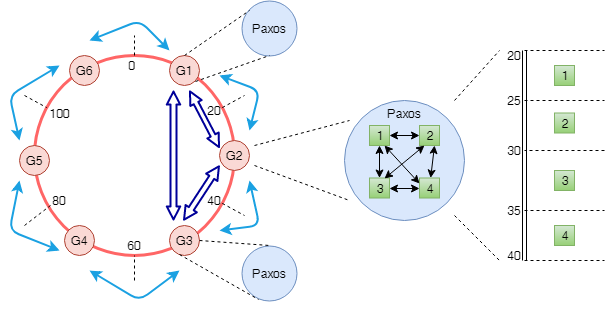
\includegraphics[width=0.8\textwidth]{image/scatterarch.png}
        \caption{Scatter Architecture}
        \label{scatterarchitecture}
    \end{figure}
    
    Figure \ref{scatterarchitecture} gives the overview of Scatter architecture. The key-space (0 - 119) is partitioned among groups (G1 to G6). The groups remain in sync with its immediate neighbours indicated by light-blue arrows. Every node in the group acts as primary node for a range of keys assigned to the group. The key range 20-39 for group G2 is divided among its nodes 1, 2, 3, 4 such that every node is a primary for a subset of that range. Multi-group transactions (groups G1, G2 and G3 in our case) use a two-phase commit protocol (indicated by dark-blue arrows). The overall technique is called nested consensus. The groups use Paxos Distributed Consensus algorithm \cite{PaxosLamport} within themselves for consistent decision making (indicated by black arrows).
    
    Scatter applies different policies to suit different operating conditions and they help to change the system behaviour without changing the mechanism. The three deployment setups taken into consideration were – Low churn and uniform network latency, low churn and non-uniform network latency, and high churn and non-uniform network latency. Some system properties which were considered and the policies which Scatter applies to ensure them are described as follows. 
    
    \begin{itemize}
        
        \item	\textbf{Resilience} A group cannot perform its operations in a safe manner if it faces failure of more than 50\% of nodes. So, to improve resilience, Scatter applies a policy which says that if the total number of nodes in a group falls below a threshold, then it should merge with other groups. This prevents data loss but affects the performance. This policy also tells how a new node joins the system. A new node samples K groups, checks their probability to fail using the node lifetime information, and then makes the decision. In case it finds more than one groups to be below that threshold, it picks the group based on the policy of optimizing latency.
        \item	\textbf{Latency} Client latency is the time taken to reach the primary, plus the time taken by primary to reach consensus with the other replicas. So, according to the latency optimization policy, the node should join a group where it has less latency with the group nodes. A new node should sample K groups by sending a no-op operation, and then decide based on the results.
        \item	\textbf{Load Balance} The policy states that a new node should join the heavily loaded group. It samples K nodes, selects groups with low failure probability, and then checks the number of operations it has processed in recent past to make the decision. The policy also states the repartitioning on a group key space among its adjacent groups if a particular range is facing heavy loads. 
        
    \end{itemize}
    
    \section{Conclusion}
    
    In this paper, we discussed distributed storage systems, how are they designed, discussing in detail the various design paradigms for efficient, reliable systems for various use cases. We discussed in detail Distributed Hash Tables, and how they address the need of a distributed storage system.
    
    We also discussed in detail five key milestone works in the field of distributed storage. Chord, as discussed in Section \ref{chord}, introduced a lookup protocol to helps efficiently locate the node in a distributed environment that stores a specific piece of data. On the other hand, Pastry (Section \ref{pastry}) is a work focused on the design of decentralized systems for peer-to-peer applications, with nodes connected via the Internet. Pastry and Chord are very similar to each other. Both of them are using circular identifier space. The sizes of lookup table that each node needs to maintain are also comparable in these two protocols. However, the routing rule of Chord is more straightforward, which is an advantage for system maintenance.
    
    Further, we discuss in Section \ref{opendht}, the landmark introduction of OpenDHT, a free, public DHT, which can be both simple to implement applications over, while also meeting a broad spectrum of application requirements.
    
    Then, Comet (Section \ref{comet}) and Scatter (Section \ref{scatter}) present distributed key-value storage systems, each with their own usage scenarios, advantages and some restrictions.
    
    \subsection{Future Research Directions}
    
    With the increasing demand for high volumes of data, driven by content streaming services like Netflix, there is a need to build systems that are able to efficiently deliver such content, with lower dependence on centralized servers, in order to improve performance and availability, while reducing costs. This can especially be advantageous in streaming sports, when a large number of people tune in at the same time. The current systems have failed to handle loads when millions of people contact the servers at the same time, for the same content. In this specific case, effort also needs to be made to minimize latency, which is one of the most important aspects of sports broadcast.
    
    \bibliographystyle{abbrv}
    \bibliography{paper}
    %{\small \bibliography{paper} }
    
\end{document}